% subject: コンピュータサイエンス第一期末試験(雛形)
% date:    18/11/21
% LaTeX2e: Japanese

\documentclass[12pt]{article}
\pagestyle{empty}
\usepackage{ascmac}
\usepackage[dvips]{epsfig}

% local.mac

%%% STYLE PARAM.s (for A4) %%%
\textwidth=16cm
\textheight=240mm

\topmargin=0mm
\headsep=0cm
\headheight=0cm
\oddsidemargin=0cm
\evensidemargin=0cm
\marginparwidth=0cm

\footnotesep=15pt
%\footheight=1.5cm
%\footskip=1.5cm

\itemsep=0.1pt
\parindent=11pt

\def\baselinestretch{1.15}

%%% LOCAL MACRO DEF.s %%%

\newcommand{\OMIT}[1]{}

% Print control (skips)
%\newcommand{\bigskip}{\vskip12pt}
%\newcommand{\medskip}{\vskip6pt}
%\newcommand{\smallskip}{\vskip3pt}
\newcommand{\paragraphskip}{\vskip\topsep}

% Itemization, etc
\newcommand{\nitem}[1]{%
\par\noindent\hangindent20pt%
\hskip20pt\llap{#1~}}
\newcommand{\nnitem}[1]{%
\par\noindent\hangindent30pt%
\hskip30pt\llap{#1~}}

\begin{document}
\noindent
\hfill{\small 21.Nov.2018}

\noindent
\hfil
{\large\bf
コンピュータサイエンス第1\textemdash 期末試験 CS4b\textemdash}
\hfil

\paragraphskip\noindent
※答案用紙は各問ごとに 1 枚使用して書くこと.\\
※答案用紙には各枚ごとに学籍番号と氏名を書くこと.

\paragraphskip
\nitem{\bf 問1.}(配点 10 点)\\
つぎの問に答えよ.計算の過程も解答用紙に残すこと.
\((n)_{m}\) は $n$ が $m$ 進表記であることを表すものとする.
  \begin{enumerate}
\item \((18)_{10}\) を 2 進表記に変換せよ.
\item \((10100)_{2}\) を 10 進表記に変換せよ.
  \end{enumerate}

\paragraphskip
\nitem{\bf 問2.}(配点 10 点)\\
Ruby 処理系で以下のように入力して結果を得たとする.
この結果を参考に図の (1)-(10) を埋めよ.
図は文字列がメモリ上に格納されている様子を示している.
  \begin{itembox}{出力例}
\textgreater "Ice\%creams".unpack("H*")\\
=\textgreater ["49636525637265616d73"]\\
  \end{itembox}
  \begin{center}
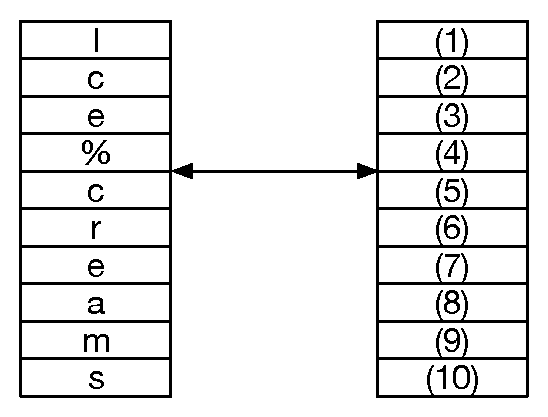
\includegraphics[scale=1.0]{./Figure/elementaryCS-figStrings_hole.eps}
  \end{center}

\hfill{裏面につづく}
\newpage
\paragraphskip
\nitem{\bf 問3.}(配点 15 点)\\
次に示したのは言語 Ruby で書かれたプログラムである.
このプログラムについて以下の問いに答えよ.
\begin{verbatim}
CODE_a = 97
CODE_z = 122
ALPHABET_SIZE =26

def letter2index (letter)
  return (letter - CODE_a)
end
def index2letter (index)
  return (index + CODE_a)
end
def transform(char,key)
  index = letter2index(char)
  c_index = (index + (letter2index(key))) % ALPHABET_SIZE
  return(index2letter(c_index))
end
def vigenere (key,message,chipher_text)
  key_length=key.length
  message_length=message.length
  for i in 0..(message_length-1)
    if CODE_a <= message[i] && message[i] <= CODE_z
       chipher_text[i] = transform(message[i],key[i % key_length])
    else
       chipher_text[i] = message[i]
    end
  end
end
def encipher(key, message)
  letters = message.unpack("C*")
  keys = key.unpack("C*")
  chipher_letters = Array.new(message.length)
  vigenere(keys,letters,chipher_letters)
  return (chipher_letters.pack("C*"))
end

angobun = encipher("vigenere", hirabun)
\end{verbatim}
\nitem{(1)}
平文 "hello" が入力として与えられたときの暗号文を示せ.
\nitem{(2)}
文字の置き換えをどのようにしているか modulo の計算式を示しながら説明せよ.

\end{document}
